\section{Metropolis Theme}

	% FRAME
	\begin{frame}[fragile]{Metropolis}
	
		The Metropolis theme is a Beamer theme with minimal visual noise
		inspired by the \href{https://github.com/hsrmbeamertheme/hsrmbeamertheme}{\textsc{hsrm} Beamer
		Theme} by Benjamin Weiss.
		
		Enable the theme by loading
		
		\begin{verbatim}
			  		\documentclass{beamer}
			   	\usetheme{metropolis}
		\end{verbatim}
		
		Note, that you have to have Mozilla's \emph{Fira Sans} font and XeTeX
		installed to enjoy this wonderful typography.
	\end{frame}

	\begin{frame}[fragile]{Sections}
		Sections group slides of the same topic
		
		\begin{verbatim}    \section{Elements}\end{verbatim}
		
		for which Metropolis provides a nice progress indicator \ldots
	\end{frame}

\subsection{Title formats}

	\begin{frame}{Metropolis title formats}
		Metropolis supports 4 different title formats:
		\begin{itemize}
			\item Regular
			\item \textsc{Small caps}
			\item \textsc{all small caps}
			\item ALL CAPS
		\end{itemize}
		They can either be set at once for every title type or individually.
	\end{frame}

	{
	\gothamset{titleformat frame=smallcaps}
	\begin{frame}{Small caps}
		This frame uses the \texttt{smallcaps} title format.

		\begin{alertblock}{Potential Problems}
			Be aware that not every font supports small caps. If for example you typeset your presentation with pdfTeX and the Computer Modern Sans Serif font, every text in small caps will be typeset with the Computer Modern Serif font instead.
		\end{alertblock}
	\end{frame}
	}

	{
	\gothamset{titleformat frame=allsmallcaps}
	\begin{frame}{All small caps}
		This frame uses the \texttt{allsmallcaps} title format.

		\begin{alertblock}{Potential problems}
			As this title format also uses small caps you face the same problems as with the \texttt{smallcaps} title format. Additionally this format can cause some other problems. Please refer to the documentation if you consider using it.

			As a rule of thumb: just use it for plaintext-only titles.
		\end{alertblock}
	\end{frame}
	}

	{
	\gothamset{titleformat frame=allcaps}
	\begin{frame}{All caps}
		This frame uses the \texttt{allcaps} title format.

		\begin{alertblock}{Potential Problems}
			This title format is not as problematic as the \texttt{allsmallcaps} format, but basically suffers from the same deficiencies. So please have a look at the documentation if you want to use it.
		\end{alertblock}
	\end{frame}
	}


\subsection{Elements}

	\begin{frame}{Blocks}
		Three different block environments are pre-defined and may be styled with an
		optional background color.
		
		\begin{columns}[T,onlytextwidth]
		 \column{0.5\textwidth}
		   \begin{block}{Default}
		     Block content.
		   \end{block}
		
		   \begin{alertblock}{Alert}
		     Block content.
		   \end{alertblock}
		
		   \begin{exampleblock}{Example}
		     Block content.
		   \end{exampleblock}
		
		 \column{0.5\textwidth}
		
		   \gothamset{block=transparent}
		
		   \begin{block}{Default}
		     Block content.
		   \end{block}
		
		   \begin{alertblock}{Alert}
		     Block content.
		   \end{alertblock}
		
		   \begin{exampleblock}{Example}
		     Block content.
		   \end{exampleblock}
		
		\end{columns}
	\end{frame}

	\begin{frame}{Presetted Plots styles}
		\begin{columns}[T,onlytextwidth]
			\column{0.5\textwidth}
			\begin{figure}
				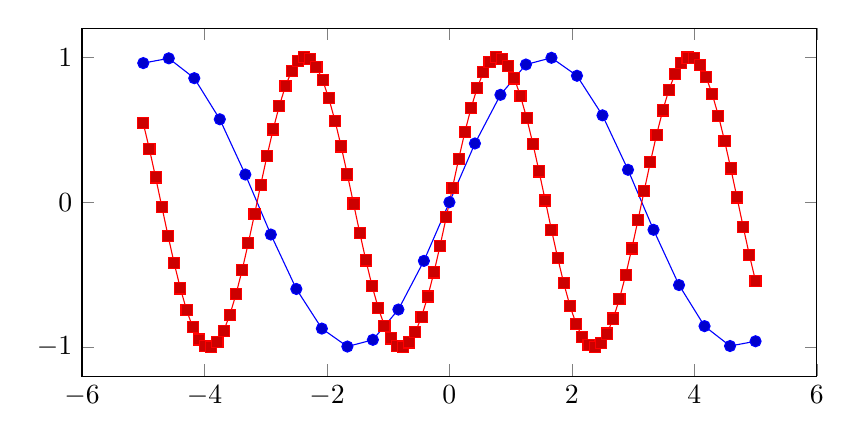
\begin{tikzpicture}
					\begin{axis}[
						%mlineplot,
						width=0.9\textwidth,
						height=6cm,
						]

						\addplot {sin(deg(x))};
						\addplot+[samples=100] {sin(deg(2*x))};

					\end{axis}
				\end{tikzpicture}
				\caption{A nice sinus plot with Tikz.}
			\end{figure}

			\column{0.5\textwidth}
			\begin{figure}
				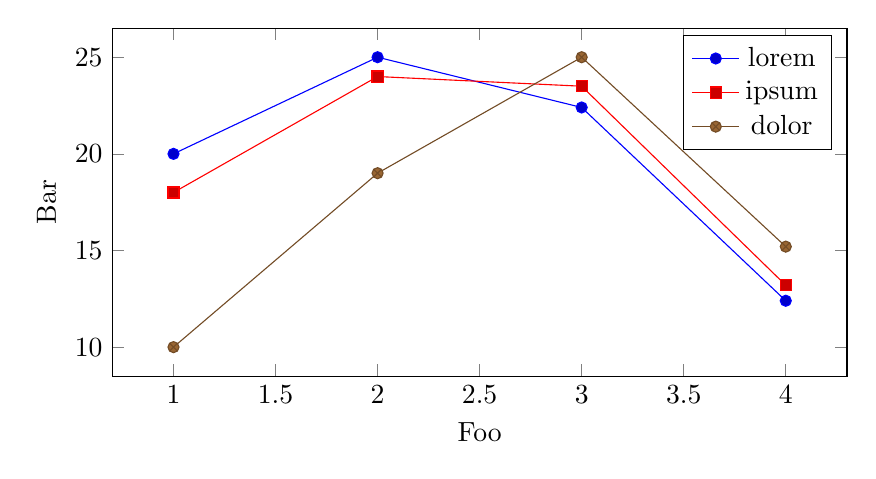
\begin{tikzpicture}
					\begin{axis}[
						%mbarplot,
						xlabel={Foo},
						ylabel={Bar},
						width=0.9\textwidth,
						height=6cm,
						]

						\addplot plot coordinates {(1, 20) (2, 25) (3, 22.4) (4, 12.4)};
						\addplot plot coordinates {(1, 18) (2, 24) (3, 23.5) (4, 13.2)};
						\addplot plot coordinates {(1, 10) (2, 19) (3, 25) (4, 15.2)};

						\legend{lorem, ipsum, dolor}

					\end{axis}
				\end{tikzpicture}
				\caption{A nice bar chart with Tikz.}
			\end{figure}
		\end{columns}
	\end{frame}

	{%
	\setbeamertemplate{frame footer}{My custom footer}
	\begin{frame}[fragile]{Frame footer}
	   Metropolis defines a custom beamer template to add a text to the footer. It can be set via
	   \begin{verbatim}\setbeamertemplate{frame footer}{My custom footer}\end{verbatim}
	\end{frame}
	}

	\begin{frame}[fragile]{Standout}
		The final slide has a new option style with command:
		\begin{verbatim}
		 \begin{frame}[standout]
	   \frametitle{Thank You !}
	     Questions ?
		 \ end{frame}
		\end{verbatim}

		\begin{center}
			Et voilà !
		\end{center}
	\end{frame}
